%label:"art:examplesOfSymplecticManifolds"
%author:JeffHicks
%name:"examples of symplectic manifolds "
%type:"article"

%label:"exm:linearSymplecticSpace"
%type:"example"
%name:"linear symplectic space"


    The simplest example comes from $\RR^{2n}$, which we give the coordinates $(q_i, p_i)$. 
    In these local coordinates, we can define a symplectic form by  
        \[\omega_{std}=\sum_{i=1}^n d p_i\wedge d q_i.\] 
    Note that when $n=1$, this gives the standard area form on $\RR^2$.
    In these coordinates, it is easy to check that $\frac{\omega_{std}^n}{n!}=\text{vol}_{\RR^{2n}}$, the standard volume form.


%label:"def:symplecticSurface"
%type:"example"
%name:"symplectic form on surfaces"


    Let $(X, g)$ be an oriented surface.
    Then $g$ prescribes a volume form $\omega:=\text{vol}_g\in \Omega^2(X;\RR)$, which is an example of a non-degenerate 2-form. 
    Because $\Omega^3(X;\RR)=0$, it trivially follows that $\omega$ is closed. 
    This example raises the possibility of the same space having many different symplectic forms, as an oriented surface can be equipped with several different metrics.


%label:"exm:ccstarcylinder"
%type:"example"
%name:"symplectic structure on Cylinder"

    An example that will be especially relevant later is $(\CC^*)^n$.
    We will equip this with a different symplectic form than the one inherited as a subset of $\CC^n=\RR^{2n}$.
    Since $(\CC^*)^n$ is a group, it is natural to ask for a symplectic form on $(\CC^*)^n$ which is invariant under the group action. 
    The symplectic form 
    \[
        \omega=\frac{1}{2\pi} d(\log |z|)\wedge d\theta
    \]
    gives an example of such a symplectic form.
When $n=1$, then this is the area form on $(\CC^*)$ which embeds into three dimensional space as an infinitely long cylinder, as drawn in \cref{fig:ccStarCylinder}.

%label:"fig:ccStarCylinder"
%author:JeffHicks
%type:"figure"
%parent:exm:ccStarCylinder
%caption:"The symplectic structure that we choose for $\CC^*$ makes it an infinitely long cylinder."

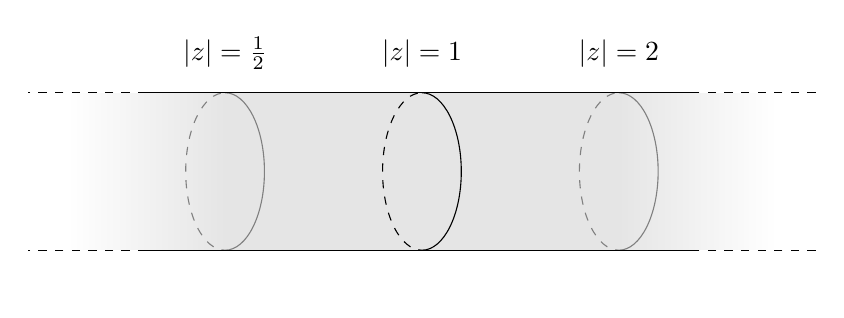
\begin{tikzpicture}

    \usetikzlibrary{fadings}
\fill[fill=gray!20, path fading = west]  (-4.5,1.5) rectangle (-2.5,-0.5);
\fill[fill=gray!20]  (-2.5,-0.5) rectangle (2.5,1.5);

\fill[fill=gray!20, path fading = east]  (4.5,1.5) rectangle (2.5,-0.5);
\begin{scope}[]

\begin{scope}[]

\clip  (0,2) rectangle (1,-1);
\draw  (0,0.5) ellipse (0.5 and 1);
\end{scope}
\begin{scope}[]

\clip  (0,2) rectangle (-1,-1);
\draw[dashed]  (0,0.5) ellipse (0.5 and 1);
\end{scope}
\end{scope}

\begin{scope}[shift={(2.5,0)}, draw=gray]

\begin{scope}[]

\clip  (0,2) rectangle (1,-1);
\draw  (0,0.5) ellipse (0.5 and 1);
\end{scope}
\begin{scope}[]

\clip  (0,2) rectangle (-1,-1);
\draw[dashed]  (0,0.5) ellipse (0.5 and 1);
\end{scope}
\end{scope}

\begin{scope}[shift={(-2.5,0)},draw=gray]

\begin{scope}[]

\clip  (0,2) rectangle (1,-1);
\draw  (0,0.5) ellipse (0.5 and 1);
\end{scope}
\begin{scope}[]

\clip  (0,2) rectangle (-1,-1);
\draw[dashed]  (0,0.5) ellipse (0.5 and 1);
\end{scope}
\end{scope}
\begin{scope}[]
\draw (-3.5,1.5) -- (3.5,1.5);
\begin{scope}[]
\draw[dashed] (-3.5,1.5) -- (-5,1.5);
\end{scope}
\begin{scope}[shift={(8.5,0)}]
\draw[dashed] (-3.5,1.5) -- (-5,1.5);
\end{scope}
\end{scope}
\begin{scope}[shift={(0,-2)}]
\draw (-3.5,1.5) -- (3.5,1.5);
\begin{scope}[]
\draw[dashed] (-3.5,1.5) -- (-5,1.5);
\end{scope}
\begin{scope}[shift={(8.5,0)}]
\draw[dashed] (-3.5,1.5) -- (-5,1.5);
\end{scope}
\end{scope}
\node at (-2.5,2) {$|z|=\frac{1}{2}$};
\node at (0,2) {$|z|=1$};
\node at (2.5,2) {$|z|=2$};
\end{tikzpicture}


The most important example of symplectic manifold comes from physics, which is the historical origin of symplectic geometry. 
%label:"def:symplecticCotangentBundle"
%type:"example"
%name:"symplectic structure on cotangent bundle"


    Let $Q$ be a smooth $n$-dimensional manifold.
    We now describe a canonical symplectic form on the cotangent bundle, $T^*Q$.
    At every point $q\in Q$, there exists chart $q\in U\subset Q$ which we can parameterize with coordinates $(q_1, \ldots, q_n)$.
    The cotangent bundle $T^*U$ inherits coordinates $(q_1, p_1, q_2, p_2, \ldots, q_n, p_n)$, where the $p_i$ linearly parameterize the fibers of the cotangent bundle in the direction of the basis element $dq_i$.
    \footnote{ The letter $p$ is chosen for historical reasons. The form $dq_i$ is dual to the vector $\partial q_i$, which represents the velocity of a particle.     The dual to velocity is momentum, which was historically represented by the variable $\rho$.    Therefore, the momentum coordinates have been denoted by $p_i$.  } 
    In these coordinates, the canonical symplectic form on this chart is:
    \[\omega=\sum_{i=1}^n dq_i \wedge dp_i=-d(p dq).\]


In the physical literature, $T^*Q$ is called the ``phase-space'' which encodes both the position and momentum of a particle.
The canonical symplectic form describes the natural pairing of momentum and velocity.
There is also a coordinate-free description of $\omega$.
 To do so, we first define a canonical 1-form  $\eta\in \Omega^1(T^*Q)$.
Let $(q,p)\in T^*Q$ be a point, where the coordinates take values $q\in Q$ and $p\in T^*_qQ$.
The map $\pi: T^*Q\to Q$ induces a map $\pi_*: T(T^*Q)\to TQ$. 
The canonical 1-form is defined by its value on tangent vectors  $v\in T_{(q,p)}(T^*M)$
\[\eta_{(q,p)}(v):=p(\pi_*(v)).\]
This describes the pairing between the $Q$-component (velocity in the base) of $v$  and the momentum coordinate $p$. 
From the canonical form, we obtain a coordinate-free definition of canonical symplectic form as 
\[\omega=-d\eta.\] 
Note that $\omega$ is not simply a closed 2-form, but rather an \emph{exact symplectic form. }  

\snip{One can also prove}{art:weinstein} that the cotangent bundle serves as a general kind of local model for symplectic manifolds. 
We've already seen the cotangent bundle appear in the examples of symplectic structures on $\RR^{2n}$ and $(\CC^*)^n$, which can be interpreted as the symplectic structures on the cotangent bundles $T^*\RR^n$ and $T^*T^n$ respectively. 
This example also gives an example of how an almost complex structure and symplectic structure can interact.
    Let $Q$ be a manifold equipped with a connection.
    The tangent bundle of $Q$ comes with an almost complex structure.
    With a choice of connection we obtain a splitting
    \[T_{(q,v)}TQ= T_v (T_q Q)\oplus T_q Q\]
    with an isomorphism $A: T_v(T_q Q)\to T_qQ.$
    One can then construct an almost complex structure by taking the matrix 
    \[J:=\begin{pmatrix} 0 & A\\ -A^{-1} & 0\end{pmatrix}: T_{(q,v)}TQ\to T_{(q,v)}TQ.\]
    One can similarly (but not canonically) construct an almost complex structure for the cotangent bundle. 
    Pick $g$ a metric for $Q$, which induces a bundle isomorphism between the tangent and cotangent bundle. 
    Let $(q_1, \ldots, q_n, p_1, \ldots p_n)$ be local coordinates for $T^*Q$ chosen so that $\partial q_1, \ldots \partial q_n$ form an orthonormal basis at the origin and the coordinates $p_1, \ldots, p_n$ parameterize the linear coordinates determined by the basis $\{\iota_{\partial q_i}g\}$.
    Then an almost complex structure is specified by 
    \begin{align*}
        J \partial q_i=\partial p_i && J\partial p_i = -\partial q_i.
    \end{align*}
    Note that the resulting almost complex structure depends on the choice of metric, which modifies the ``size'' of the cotangent fiber relative to the base. 
    The metric $\omega(J, -)$ is then the standard induced metric on the cotangent bundle.